% mainfile: ../../../../master.tex
\subsection{Nucleic acids quantification with NanoDrop spectrophotometer}
% The part of the label after the colon must match the file name. Otherwise,
% conditional compilation based on task labels does NOT work.
\label{task:20180208_cj0}
\tags{lab,dna,rna,qnt}
\authors{cj}
%\files{}
%\persons{}

\sidenote{As absorbance measurements will measure any molecules absorbing at a specific wavelength, nucleic acid samples will require purification prior to measurement to ensure accurate results. Nucleotides, RNA, ssDNA, and dsDNA all will absorb at 260 nm and contribute to the total absorbance.}

\begin{figure}[H] % position of the figure 
    \centering
    \caption{Screen captures of the measurements by NanoDrop spectrophotometer}
    \label{fig:CJ20180208_ALLPREP}
    \begin{subfigure}[b]{0.49\textwidth}
        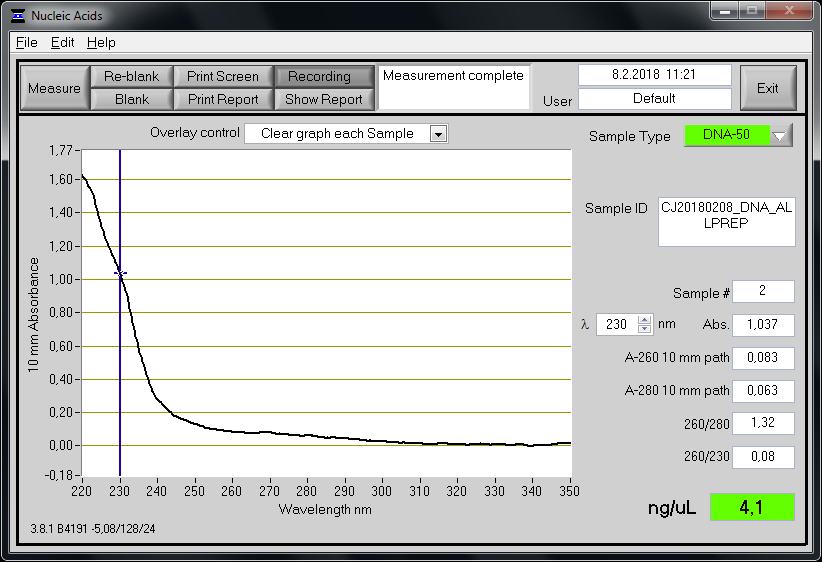
\includegraphics[width=\textwidth]{graphics/screenshots/CJ20180208_DNA_ALLPREP.png}
        \caption{Measurments for DNA extracted with the AllPrep kit}
        \label{sfig:CJ20180208_DNA_ALLPREP}
    \end{subfigure}
    ~ 
    \begin{subfigure}[b]{0.49\textwidth}
        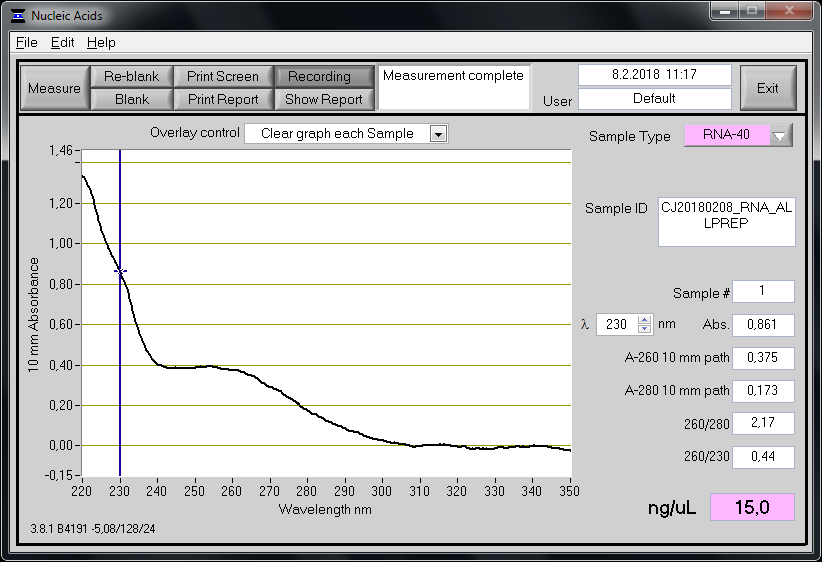
\includegraphics[width=\textwidth]{graphics/screenshots/CJ20180208_RNA_ALLPREP.png}
        \caption{Measurments for RNA extracted with the AllPrep kit}
        \label{sfig:CJ20180208_RNA_ALLPREP}
    \end{subfigure}
\end{figure}

\begin{table}[htbp]
\caption{res/nanodrop/CJ20180208.txt}
\label{tab:CJ20180208}
\centering
\begin{tabular}{l l l l l l l l l l l l l }
\toprule
Sample ID & Time  & ng/ul  & A260  & A280  & 260/280  & 260/230  \\ \midrule
\texttt{CJ20180208\_DNA\_ALLPREP} & 11:21 & 4,1 & 0,083 & 0,063 & 1,32 & 0,08  \\
\texttt{CJ20180208\_RNA\_ALLPREP} & 11:17 & 15,0 & 0.375 & 0,173 & 2,17 & 0,44 \\
\bottomrule
\end{tabular}
\\
User: Default - Date: 08.02.2018 - Constant: 33,00 - Cursor position: 230 \
\end{table}

The ratio of absorbance at 260 nm and 280 nm is used to assess the purity of DNA and RNA. A ratio of \~1.8 is generally accepted as "pure" for DNA; a ratio of \~2.0 is generally accepted as "pure" for RNA. If the ratio is appreciably lower in either case, it may indicate the presence of protein, phenol or other contaminants that absorb strongly at or near 280 nm.

For my DNA, the 260/280 ratio value is 1.32 which is lower than the expected 1.8 for "pure" DNA. The curve in figure \ref{sfig:CJ20180208_DNA_ALLPREP} indicates contamination with compounds with absorbance near 230 nm like \gls{edta}, carbohydrates and phenol. Here I did not use phenol and I made sure not to use TE buffer to resuspend my DNA pellet, so it could be contaminated with carbohydrates.

For my RNA, the 260/280 ratio value is 2.17 which is suprisingly higher than 2.0 which is considered as "pure" RNA.

For my first attenmpt with the AllPrep DNA/RNA Mini Kit, the results are not convincing. It would be due to my inexperience with this kit, or also because the kit expired in 2011. I can still try to amplify the DNA and later, I would repeat an extraction with this kit and maybe use the beta-mercapto ethanol as it is suggested in the instructions.


